\documentclass{IEEEtran}
\usepackage[utf8]{inputenc}
\usepackage[english]{babel}
\usepackage{hyperref}
\usepackage{amsmath}
\usepackage{graphicx}
\usepackage{csquotes}
\usepackage{multirow}
\usepackage{graphics}
\graphicspath{{./images/}}
\usepackage[style=nature]{biblatex}
\addbibresource{references.bib}

\title{Generating Americana with transfer learning from the music transformer \\
    \normalsize{\url{github.com/gregwinther/folk_transformer} and \url{https://gregwinther.github.io/folk_transformer/}}}

\author{\IEEEauthorblockN{Sebastian G. Winther-Larsen} \\
\IEEEauthorblockA{\textit{Center for Computing in Science Education,
    Department of Physics, University of Oslo} \\
}
\and
\IEEEauthorblockN{Tom F. Hansen} \\
\IEEEauthorblockA{\textit{Institute of Informatics, University of Oslo} \\
}
\and
\IEEEauthorblockN{Bjørn Iversen} \\
\IEEEauthorblockA{\textit{Institute of Informatics, University of Oslo} \\
}
}


\begin{document}
    \maketitle

    \begin{abstract}
        Since the publication of the music transformer in 2018, music generators based on
        the transformer architecture has been state of the art, making it possible to generate
        realistic music for minutes. Up to now the results have mainly been succesful for piano music, but
        have failed for more technically complex music such as jazz. Americana folk music can be seen as
        a stepping stone to more complex music. In this work we generate Americana folk music with 2 different approaches; transfer learning from the MAESTRO dataset and solely traning on the Americana dataset. We then evaluate these results in a qualitative and quantitative way. Results from the 
        quality assessment indicate that both models have been moderately succesful, and the model based on transfer learning is favoured. In a rating process people have rated the songs to in averate 2.5,
         where 1 is not realistic and 5 is realistic, compared to "real" humanmade music. In a technical 
         evaluation the evaluated songs showed a....
        \end{abstract}
        
        \begin{IEEEkeywords}
        music generation, transformer model, evaluation, transfer learning, Americana
        \end{IEEEkeywords}

    \section{Motivation and introduction}

        The attention-based transformer model,
        is today recognised as the best performing sequential machine learning model,
        surpassing RNN-based models in most cases, mainly argued by its better abilities
        to remember long term coherence, shorter training time and applicability in transfer
        learning~\cite{vaswani2017attention}.
        While originally used primarly for
        natural language processing (NLP), which today has mature implementations,
        the architecture can also be applied for other sequential models,
        such as music generation~\cite{huang2018music}.
        The music transformer developed in the Magenta project is trained on the Maestro
        dataset~\cite{maestrodataset}.
        By setting a primer – a start music sequence, the model generates new music with good
        results along the same lines as the training set. With other primers than regular and
        systematic classical music in Maestro, the quality of the output is varying.
        
        Motivated by generating more irregular music, the main aim of the paper is
        to describe a framework for the quality assessment of different approaches to the generation 
        of music with the transformer model. By building, what is supposed to be the same 
        music generator, but with different approaches, the evaluation framework will assess 
        the quality of each approach. It is not known to the authors scientific papers
        describing such a comparison of music transformers, other than the normal
        comparison of music generated by RNNs and transformers ~\cite{huang2018music}.
        At the core of such an architecture is, for each approach; 1) in order to make a fair comparison,
        a detailed description of model topology, its tuning parameters, and the size
        and structure of the dataset used for training, and 2) an evaluation format
        that combines a form of quantitative and qualitative evaluation technique.
       
        To this end, we wish to employ the transformer music to a subgenre of music   
        to which such a model has not been extensively applied.
        While initial findings from applying the transformer to jazz music has shown 
        some limitations~\cite{wu2020jazz}, while applying LSTM networks to Blues has 
        been moderately succesful~\cite{eck2002bluesLSTM} and applying the transformer 
        model to pop music seems to work well~\cite{huang2020pop}.
        From a music theory standpoint this is very sensible - classical music often has 
        formal rules, the epitome of which is the fugue~\cite{giraud2015computational};
        and pop music follows some very clear norms~\cite{hennion1983production}. While 
        even Free Jazz has \emph{some} rules, it readily falls into the category of the 
        type of rhytmic music with the least amount of structure, per the definition
        that it is ``characterized by the absence of set chord patterns or
        time patterns''\cite{FreeJazz}.

        American roots music, encompassing spirituals, cajun music, cowboy music, work songs,
        but also early blues such as Dixieland; from now on referred to as ``Americana'', presents 
        itself as hitherto unexplored territory. It also provides a nice stepping stone
        towards more ``unstructured'' music as it often allows for improvisationg, but 
        otherwise retains a relatively rigid structure~\cite{libcong}.
        We have therefor collected a dataset of MIDI files of Americana music, which we
        will use in our quality assessment framework.

    \section{Related work}
       The transformer model is considered state of the art in music generation,
       surpassing RNN-based models in the last few years. Both are sequential models,
       but the attention principle at the core of the transformer facilitates
       remembering coherence over longer sections of sequences and highlights
       especially important sections. From generating music of 10's of seconds with RNN, it is now possible to generate a minute of coherent realistic music ~\cite{huang2018music}. Still there is a lot of unresolved challenges, like generating long sections (over some minutes), in highly irregular compositions
       and multi channel (many instruments) signals. To combat these challenges the
       improvement of the transformer model has high focus in the research community.
       Some of the most recent attempts are the Transformer-XL~\cite{dai2019transformerxl} 
       model and the Reformer~\cite{kitaev2020reformer} as particularly promising
       candidates.
       A Reformer model claim to be trained on a standard computer with a single GPU.
       In this analysis we will utilize the original transformer architecture, as this
       is the model-architecture in the music transformer from Google.

       \subsection{Music transformers}
       In the few existing papers considering music generation with the Transformer
       we want to emphasize some important related works besides the beforementioned
       music transformer, built on the classical piano music dataset MAESTRO.
       These works are somewhat diversified in different music genres. In the pop
       music transformer \cite{huang2020pop} pop piano music is generated by the
       transformer. The paper shows that Transformers can do even better for music
       modeling, when the way a musical score is converted into the data fed to a
       Transformer model, is improved. This is performed by imposing a metrical structure
       in the input data, so that Transformers can be more easily aware of the
       beat-bar-phrase hierarchical structure in music. The new data representation
       maintains the flexibility of local tempo changes, and provides hurdles to control
       the rhythmic and harmonic structure of music. With this approach, this work
       claims to generate pop piano music with better rhytmic structure than the music
       transformer \cite{huang2018music}.

       Another paper describes the Jazz transformer~\cite{wu2020jazz} which is in the
       other end of the spectrum related to complexity. Here the the Transformer-XL
       architecture is utilized to model lead sheets of jazz music. Moreover, the model
       endeavors to incorporate structural events present in the Weimar Jazz Database
       (WJazzD) for inducing structures in the generated music. Even though the training
       loss values are low, the esults are not impressive. Listening tests shows a clear
       gap between the ratings of the generated and real compositions. The work analyses
       the missing parts and presents a prediction system which in an analytical manner
       shed light on why machine-generated music to date still falls short of the artwork
       of humanity. This includes analyzing the statistics of
       the pitch class, grooving, and chord progression, assessing the structureness of
       the music with the help of the fitness scape plot, and evaluating the model’s
       understanding of Jazz music.

       In a system called LakhNES~\citeauthor{donahue2019lakhnes},
       generate multi-instrumental music with the transformer~\cite{donahue2019lakhnes}.
       Their success of music generation with the piano score generation is partially
       explained by the large volumes of symbolic data readily available for that domain.
       They leverage the recently-introduced NES-MDB dataset of four-instrument scores
       from an early video game sound synthesis
       chip\footnote{The Nintendo Entertainment System (NES)}.
       They found this data to be well-suited to training with the
       Transformer architecture. The model was further improved with a pre-training
       technique to leverage the information in a large collection of heterogeneous music,
       namely the Lakh MIDI dataset. By performing transfer learning on the NES-MDB dataset,
       both the qualitative and quantitative performance from the target dataset was
       significantly improved.
       
        \citeauthor{gan2020foley} use
        the transformer architecture to generate music, but with another approach.
        In a system called Foley Music they synthesize music from a silent video about
        people playing instruments~\cite{gan2020foley}.
        A relationship between body keypoints and MIDI recordings is established.
        Music generation is then formulated as a motion-to-MIDI translation problem,
        represented with a graph transformer framework that predict MIDI from motion.
        By testing the generator on different music performances the results is proven to outperform several existing systems in music generation.

        However, there is little work on generating intentionally the same music generator
        with different approaches. Another new approach is to use transfer learning from
        an existing high performance music model.

        \subsection{Evaluation of ML-generated music}
        In the evaluation of models of music generation based on machine learning we
        would like to point out the works by \citeauthor{1030094}~\cite{1030094},
        \citeauthor{yang2020evaluation}~\cite{yang2020evaluation}
        and \citeauthor{wu2020jazz}~\cite{wu2020jazz}.
        These works describe either a qualitative evaluation or a qualitative evaluation.
        In our attempt we combine these 2 approaches and establish a common framework.

    \section{Methods}

        Acting as a base and for exemplification of the benchmark architecture,
        Americana music is generated in 2 different model concepts:
        \begin{enumerate}
            \item Utilize transfer learning with MAESTRO music transformer as a base,
                    and train with the full dataset of Americana midi-files (hereafter called Transfer Americana).
            \item Train a new transformer model only using the full Americana dataset (hereafter called Americana)
        \end{enumerate} 
        
        The hypothesis is that concept number 1 will result in the best performing model,
        but an important issue is what makes up the best model and how to evaluate such a
        subjective "sequence-result" as music in a fair and trustworthy manner? 
        Some will say this is an impossible task ~\cite{1030094}. Will a transfer learning model be significantly better than only training on a single dataset, such as has been shown in other ML-applications, like image classification \cite{7404017}, even though the MAESTRO dataset is totally different from the Americana dataset.

        An attempt to sort this out is by evaluating in a quantitative and qualitative way.
        The quantitative, hence objective, way can shortly be described as a technical
        comparison of the predicted signal and the real signal. Principles by \cite{yang2020evaluation} and ~\cite{wu2020jazz} will be utilized.
        
        The qualitative part constitutes a music expert judgement,
        based on listening to the generated music files from the objective evaluation.
        In a second, and survey based part, a number of random people is asked
        to rate the different music files.
        
        \subsection{Qantitative evaluation}
        
        For quantative evaluation we will be using the objective
        evaluation toolbox mgeval~\cite{yang2020evaluation}.
        The toolbox lets us extract absolute metrics from MIDI files
        which lets us inspect the properties of both the dataset used
        for training and the generated dataset. The features extracted
        for absolute measures are divided into pitch-based features Pitch count (PC),
        Pitch class histogram (PCH), Pitch class transition matrix (PCTM),
        pitch range (PR) and Average pitch interval (PI) and rhythm-based features,
        Note count (NC), Average inter-onset-interval (IOI), Note length
        histogram (NLH) and Note length transition matrix (NLTM).
        These metrics can then be used to acquire the relative metrics between
        datasets with the use of exhaustive cross validation to acquire the
        distance between each sample of same set (intra-dataset) and another
        set (inter-dataset). 
        
        \subsection{Evidence-Based Design for Assessment and Evaluation}
        As a rigorous and well-proven approach do construct a framework for 
        assessing music composed by artificial intelligence models, we propose 
        adapting the methodology of Evidence-Centered
        Design~\cite{mislevy2003focus,mislevy2017evidence}
        By working with Evidence-Centered Design (ECD), we engage in a modern
        approach to assessment design,
        for assessing complex knowledge and practices.
        ECD is originally applied to the contruction of psychometric learning
        assessment tools. Through to completion, it would take several years to 
        construct such a tool, something that is well outside the scope of this 
        study. However, we prospose to begin with the first step within ECD - 
        \textbf{Domain Analysis}. This involves exploratory interviews of experts
        in the field in order to contruct a thematically organized and prioritized
        list of knowledge and practices to assess. Scecific to our study,
        we find it necessary to talk to professional musicians and composers 
        in order to uncover what actually makes a good composition.
        
        \subsection{Qualitative evaluation}
        In the survey part people were presented to 5 generated songs with length 
        40 seconds - 1 minute, facilitated in a Google survey form. The songs were generated by sending a primer of the first 3 bars (xxx seconds) of 5 different original songs from the Americana dataset to the trained model. Each song were 
        presented in 2 versions, one generated  by Transfer-Americana and one by Americana. 
        They had to choose the one they liked best in each pair of songs. In addition they 
        had to rate the best version related to how realistic it was compared with human 
        generated music. The range was 1-worst to 5-best.

        3 music experts were presented to the 5 same genereated songs, and evaluated 
        the result in the form of an interview. Their background was....
        %TODO: sebastian sier du mer om hvordan dette foregår + fyller ut her

    \subsection{Datasets}

        A brief summary of each of the datasets we have used in this study 
        can be found in \autoref{tab:data}.

        \textbf{MAESTRO}~\cite{maestrodataset}
        (MIDI and Audio Edited for Synchronous TRacks and Organization)
        is a dataset with over 200 hours of virtuosic piano perfomances captured with 
        a fine alignment of approximately 3ms between note lables and audio waveforms.

        The data is a produce from performances in the International Piano-e-competition.
        During each installment of the competiton, virtuoso pianists perform on Yamaha
        Disklaviers which, in addition to being concert-quality acoustic grand pianos,
        utilize integrated high-precision MIDI capture and playback.
            
        Since the \textbf{MAESTRO} dataset contains MIDI recordings from competions, 
        the pieces are from a select set for each year. This means that many of the 
        pieces are the same, but may includes much variation within each
        performer's interpretation of the piece. 

        The \textbf{Americana} dataset is constructed from musical scores by 
        Benjamin Robert Tubb\footnote{These were scraped from a webpage that has 
        since been taken down. Consequently, we are unable to provide a proper 
        reference}. These scores are in the public domain and composed between
        the ealry 1800s and 1922. The genres range from blues, ragtime, naval songs,
        hyms, minstres songs and spirituals. 
    
        \begin{table}
        \begin{center}
            \caption{Data set description \label{tab:data}}
            \begin{tabular}{l c c c} \hline
                & MAESTRO v2 & Americana \\ \hline\hline
            No. of songs & 1282 & 5711 \\ \hline
            Total time [hours] & 201 & 329 \\ \hline
            Mean length [min] & 9.4 & 3.45  \\ \hline
        \end{tabular}
        \end{center}
        \end{table}

    \subsection{Modelling process}
        MIDI-files was first preprocessed to fit into the format used by the transformer model.
        This was carried out by utilizing an implementation of a transformer adapted for music, 
        incorporated in a package from Musicautobot \cite{musicautobot}. Scripts for transfer learning and
        single learning were built around this package. Both models were then trained on a supercomputer
        with the following specification for xxx hours:
        %TODO: sebastian fyller du inn

    \section{Results}

    \subsection{Quantitative evaluation}
        \begin{table}[]
            \begin{center}
            \caption{
                Results from quantitative evaluation
                \label{tab:data}
            }
            \begin{tabular}{l|rr|rr|rr}
            \multirow{3}{*}{} &
            \multicolumn{2}{c|}{Training} &
            \multicolumn{2}{c|}{Americana} &
            \multicolumn{2}{c}{Transfer} \\ \cline{2-7} 
            &
            \multicolumn{2}{c|}{Intra-set} &
            \multicolumn{2}{c|}{Intra-set} &
            \multicolumn{2}{c}{Intra-set} \\ \cline{2-7} 
            &
            \multicolumn{1}{c|}{mean} &
            \multicolumn{1}{c|}{STD} &
            \multicolumn{1}{c|}{mean} &
            \multicolumn{1}{c|}{STD} &
            \multicolumn{1}{c|}{mean} &
            \multicolumn{1}{c}{STD} \\ \hline
            PC   & 11.777  & 1.700  & 3.577  & 0.636 & 6.466  & 0.706 \\
            NC   & 442.377 & 73.911 & 11.377 & 1.542 & 21.955 & 4.678 \\
            PCH  & 0.384   & 0.013  & 0.164  & 0.007 & 0.365  & 0.026 \\
            PCTM & 821.396 & 56.336 & 10.475 & 0.292 & 25.991 & 3.303 \\
            PR   & 19.088  & 1.638  & 5.266  & 0.611 & 10.400 & 2.038 \\
            PI   & 3.836   & 0.510  & 0.848  & 0.128 & 2.032  & 0.479 \\
            IOI  & 0.046   & 0.006  & 0.105  & 0.007 & 0.235  & 0.022 \\
            NLH  & 0.471   & 0.027  & 0.263  & 0.022 & 0.466  & 0.043 \\
            NLTM & 316.896 & 23.442 & 23.241 & 1.359 & 46.778 & 4.027
            \end{tabular}
            \end{center}
            \end{table}

            \begin{figure}
                \centering
                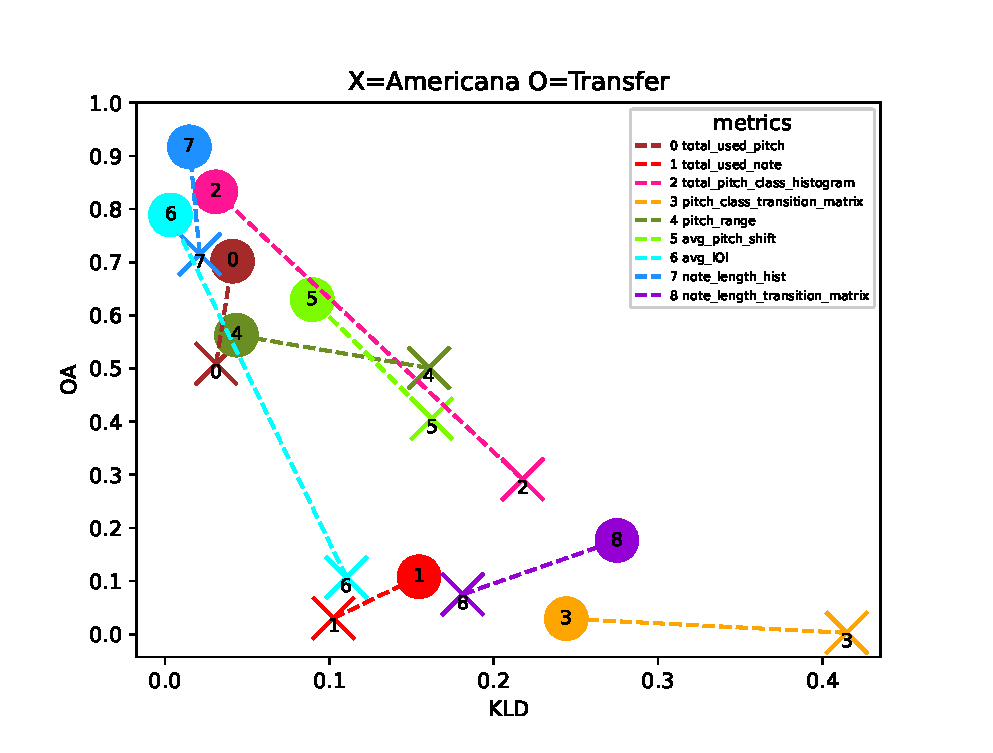
\includegraphics[width=8.5cm, height=5cm]{gen_intra_gen_training_inter}
                \caption{some label}
                \label{fig:gen_intra_gen_training_inter}
            \end{figure} 
            
            \begin{figure}
                \centering
                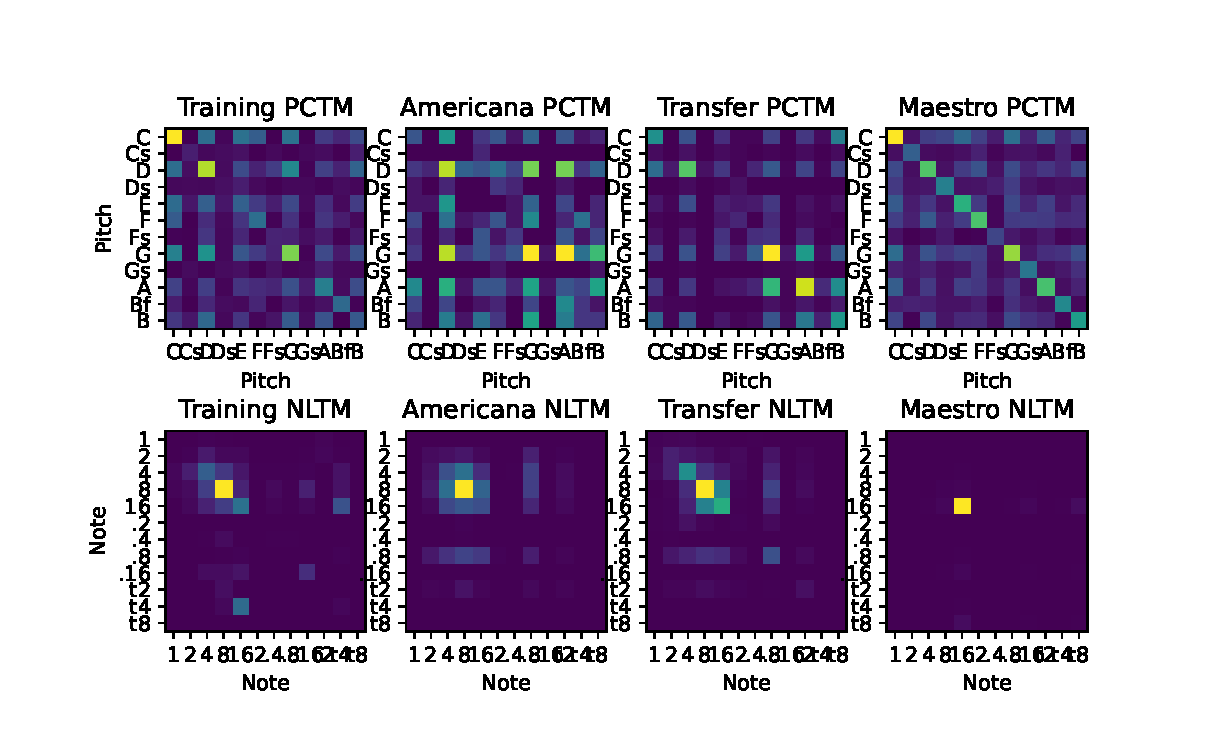
\includegraphics[width=8.5cm, height=5cm]{PCTMNLTM.eps}
                \caption{some label}
            \end{figure} 
            
        %TODO: Bjørn: Lager du en tekst til dette kapittelet.

    \subsection{Qualitative evaluation}
    
        \begin{figure}[h]
            \centering
            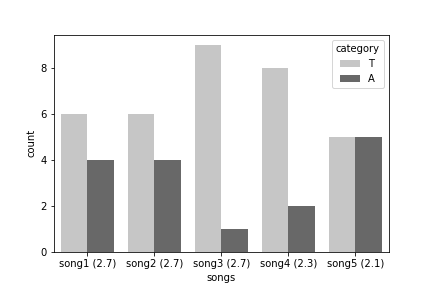
\includegraphics[width=8.5cm, height=5cm]{songs_category.png}
            \caption{Bars show a count of the number of votes, respectively for Transfer-Americana
             and Americana, for each of the 5 songs. The numbers in parenthesis below the Bars
             is the average rating for each of the songs, when compared to a realistic human made
             song (1 is worst, 5 is best)}
             \label{fig:songs}
        \end{figure} 
        Figure \ref{fig:songs} visualize a count of the number of votes, respectively for Transfer-Americana
        and Americana, for each of the 5 songs. The numbers in parenthesis below the Bars
        is the average rating for each of the songs, when compared to a realistic human made
        song (1 is worst, 5 is best). Inspecting the figure we see a general trend where Transfer-Americana is
        favoured in 4 of 5 songs. Song 5 has equal score, but is also the song with the lowest 
        realistic-rating. A t-statistic was calculated for this result, describing a significant favouring of 
        Transfer-Americana, with a p-value of 0.07. These results verified the hypothesis that a music transformer model will perform better when it is based on the pretrained model, increasing the total number of music-samples, even though the base model was trained on the classical \textbf{MAESTRO} dataset. It must be pointed out the uncertainty related to the relatively low number of samples in the survey. 
        
        In this survey some people have made comments about the overall performance ....

        Evaluation carried out in interview with musicians resulted in.... %TODO: Sebastian

    \section{Discussion}
    When we compare the results from the quantitative and qualitative evaluation we see the same trend ..

    An interesting pattern is the variation in count of superiority between songs. In song 1, 2 and 5 the count is close to similar, but for song 3 and 4 the majority of people choose the Transfer-Americana. When we compare this to the technical evaluation we see the same pattern.... It could be that the composition and complexity in certain primers is more dependent on a bigger database of trained songs, than other primers. This is something to further analysis i future work.

    
    \section{Conclusions and further development}

    \vfill
    \pagebreak
    \printbibliography
\end{document}
